\documentclass[aspectratio=169]{beamer}
%\setbeameroption{show notes}

\usepackage{beamer_pre}


\title{Thesis meeting 2024/05/23}
\author{Albert R. S. Garde}
\date{\today}
	

\begin{document}

\frame{
	\maketitle
}

\begin{frame}[fragile=singleslide]
	\frametitle{Progress since last meeting}
    \begin{itemize}
        \item Looked into the literature.
        \item Investigated tasks for the models to solve.
    \end{itemize}
\end{frame}
\begin{frame}[fragile=singleslide]
    \frametitle{Literature}
    \begin{itemize}
        \item Failed to find literature that seemed directly relevant.
        \item Found early work talking about SAE-like things, including in biology.
        \item Found alternative interpretable units to SAE-features. Out of scope for this thesis, but probably worth mentioning.
        \item 
    \end{itemize}
\end{frame}
\begin{frame}[fragile=singleslide]
    \frametitle{Tasks}
    \begin{itemize}
        \item \verb|gelu-11| is far too underpowered for any task.
        \item The largest model we can comfortably work with is \verb|gpt2-small|, the largest we can practically work with is \verb|gpt2-xl|, and thats something of a stretch.
        These models are still underpowered for many interesting tasks.
        \item A possible task is correctly continuing the string \verb|The cat is sm| by completing a word.
        \item Basically all models can do this task, and I expected removing neurons activting on \verb|sm| to make the task harder, but this is not the case.
    \end{itemize}
    \begin{center}
        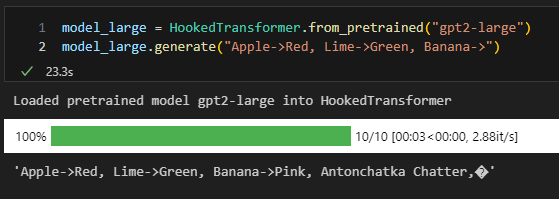
\includegraphics[scale=0.6]{images/fruit_colors.png}
    \end{center}
\end{frame}
\begin{frame}[fragile=singleslide]
    \frametitle{Plan for the next weeks}
    \begin{itemize}
        \item Continue literature review.
    \end{itemize}
\end{frame}
\begin{frame}[fragile=singleslide]
    \frametitle{Topics for meeting}
    \begin{itemize}
        \item Can we find other tasks?
        \item Investigate universality hypothesis?
        \begin{itemize}
            \item Do features with the same graphs appear in many different models?
            \item Does this differ between looking at MLP neurons and SAE features?
            \item We will need to define what we mean by "same graph".
        \end{itemize}
    \end{itemize}
\end{frame}

\end{document}